\chapter{UPPAAL and Formal Verification}\label{chap:upp}
\chapter{Semantics}\label{chap:semantics}
%!TEX root = ../../master.tex
In this chapter we describe and formalise the language \jcl, which contains a variation of the core instructions of the Java Card bytecode language. In this context the term core describes the basic set of instructions from which all other Java Card instructions can be built. 
We created this language because it is easier to model the fewer instructions in this language, rather than all the instructions in Java Card.
The full set of Java Card instructions can be built from combinations of the instructions in \jcl.
Furthermore, there exists no official formal semantics for the Java Card language.
The instructions of \jcl are defined as:
\begin{align*}
  Instructions = \{
  & \texttt{NOP}, && \texttt{PUSH } v, && \texttt{POP}, \\ 
  & \texttt{ADD}, && \texttt{DUP}, && \texttt{GOTO } a, \\ 
  & \texttt{IF\_CMPEQ } a, && \texttt{INVOKESTATIC } mid, && \texttt{RETURN},\\ 
  & \texttt{PUTSTATIC } fid, && \texttt{GETSTATIC } fid, && \texttt{LOAD } a, \\
  & \texttt{STORE } a, && \texttt{INVOKEVIRTUAL } mid, && \texttt{PUTFIELD } fid,\\ 
  & \texttt{GETFIELD } fid, && \texttt{NEW } ci && \}
\end{align*}

$\mathbb{N}$ is defined as the set of all natural numbers, including zero, and $\mathbb{Z}$ is defined as the set of all integers.
In the operational semantics we want to describe values as an integer between a minimum value and a maximum value, $Values = \{ x | x \in \mathbb{Z} \wedge x \geq \texttt{INT\_MIN} \wedge x \leq \texttt{INT\_MAX} \}$.
In addition we want a notion of addresses which is used to refer to an instruction in a method and mapping to the heap: $Addresses  = \mathbb{N}$.
A program counter is used to represent the current address $ProgramCounters = PC = Addresses$. Instructions with parameters, such as \texttt{PUSH } $v$, increment the program counter with more than one, since it uses more than one byte. \\

The program is a sequence of instructions, we denote a program as $P = (i_0, \ldots, i_k)$ where $k$ is the number of instructions in the program. 
A program consist solely of instructions $P \in Programs$ and $Programs =  \{ x | x \in Instructions^{*} \}$.
To access instructions we introduce a function accepting a program, method identifier, and a program counter. 
It returns the instruction in the method of the program at the program counter.
The function is defined as:
$$inst = Programs \times MethodID \times PC \to   Instructions$$
$$MethodID = \mathbb{N}$$

To describe a running program we use configurations.
A configuration is a 4-tuple consisting of a program, constant pool, heap and a call stack. 
$$Conf = Program \times ConstPool \times Heap \times CallStack$$
Executing an instruction means moving from one configuration to another. 
We will use $\vdash$ to indicate no change in the elements left of $\vdash$. 
For the semantic rules, no change will occur in program and constant pool e.g.:
$$CP, P \vdash \langle H, CS \rangle \rightarrow \langle H', CS' \rangle$$
Where $CP \in ConstPool$, $H,H' \in Heap$, and $CS, CS' \in CallStack$.
We use a shorthand dot notation to access elements of a tuple e.g. $conf.Program$ where $conf \in Conf$, indicates the program used in the configuration $conf$.\\

The heap can be described as a function which takes a heap address and returns either the address \textit{or} value associated with that address $Heap = Addresses \to   (Addresses + Values)_\perp$. $\perp$ represents an undefined value, and is included to describe that $Addresses$ can also map to undefined addresses/values in the heap.\\

The call stack is used to keep track of the current method scope, it is a sequence of stack frames $CallStack = StackFrames^{*}$.
A stack frame holds the method id, local variables, operand stack and the program counter for the method.

$$StackFrame = MethodID \times Locals \times OpStack \times PC $$

Local variables are represented by the function $Locals = \mathbb{N} \to   Values_\perp$. 
The operand stack is a sequence of values and addresses $OpStack = (Values + Addresses)^{*}$. \\

To represent objects we need classes in our language.
We represent classes as a 2-tuple with a possible super class and a function for resolving methods: $Class = Class_\perp \times Methods$.
$Class_\perp$ is the super class or $\perp$ in the case of no super class  
$Methods$ is the set of all method identifiers implemented by the class.
Object are represented by a 2-tuple with the class and fields of the object: 
$$Object = Class \times Fields$$ 

Fields is a function for resolving the values of class variables:
$$Fields = FieldID \mapsto (Values + Addresses)$$ 
$$FieldID = \mathbb{N}$$

Finally we make use of a constant pool to resolve static method ids, fields of static classes and class definition when creating new objects:
$$CP = ConstPool = (MethodID \to \mathbb{N}) + (FieldID \to Addresses) + (ClassIndex \to  Class)$$
$$ClassIndex = \mathbb{N}$$

%%% Local Variables:
%%% mode: latex
%%% TeX-master: "../../master"
%%% End:

\section{Instruction Semantics}
In the following semantics we make use of these abbreviation:
\begin{subequations}
\begin{align*}
H, H' &\in Heap  & CS &\in CallStack & ops, ops', ops'' &\in OpStack\\
mid, mid', mid'' &\in MethodID & loc, loc' &\in Locals & pc, pc' &\in PC\\
v &\in Values & a, objr &\in Addresses & fid &\in FieldID \\
obj, obj' &\in Object & cl &\in Class
\end{align*}
\end{subequations}
%!TEX root = ../../master.tex


\subsection{NOP}
%This instruction has no effect other than incremented $PC$ by one.
The instruction has no other effect than incrementing the $pc$.
%The no operation (NOP) instruction does nothing. Therefore only the program counter, $PC$, is incremented to point to the next instruction to be executed. Additionaly, it should also be checked whether the instruction we are currently executing is indeed a NOP. This is done with $inst(P, mid, pc) = \texttt{NOP}$\\

%This results in a changed program counter, but an unchanged stack. The operational semantics for the NOP instruction are then as follows:
%$$\inference[NOP]{PC' = PC + 1 \semsp inst(P, PC) = \texttt{NOP}}{CP, P \vdash \langle PC, S \rangle \Rightarrow \langle PC', S \rangle}$$\\

$$\inference[NOP]{inst(P, mid, pc) = \texttt{NOP}}
% % % % % % % % % % % % % % % %
{CP, P \vdash \langle H, (CS, \langle mid, loc, ops, pc \rangle)\rangle \Rightarrow 
 \langle H, (CS, \langle mid, loc, ops, pc + 1 \rangle)\rangle
}$$

%{CP, P \vdash \langle PC, S \rangle \Rightarrow \langle PC', S \rangle}$$\\

%%% Local Variables:
%%% mode: latex
%%% TeX-master: "../../master"
%%% End:

\subsection{PUSH}
\texttt{PUSH} $v$ is used to add the value from the parameter $v$ onto the top of the operand stack. Since the \texttt{PUSH} $v$ instruction takes up two bytes due to the parameter, $pc$ is incremented by two.
$$\inference[PUSH]{
inst(P, mid, pc) = \texttt{PUSH }v \semnl\\
 ops = (x_0,\ldots,x_n) \semsp ops' = (x_0, \ldots, x_n, v) \ }
{CP, P \vdash \langle H, (CS, \langle mid, loc, ops, pc \rangle)\rangle \Rightarrow
 \langle H, (CS, \langle mid, loc, ops', pc + 2 \rangle)\rangle}$$\\

\subsection{POP}
This will remove and discard the top element of the operand stack.

$$\inference[POP]{
inst(P, mid, pc) = \texttt{POP} \semnl \\
ops = (x_0, \ldots, x_{n-1}, x_n) \semsp 
ops' = (x_0, \ldots, x_{n-1})}
{CP, P \vdash \langle H, (CS, \langle mid, loc, ops, pc \rangle)\rangle  \Rightarrow \langle H, (CS, \langle mid, loc, ops', pc + 1 \rangle)\rangle}$$

\subsection{ADD}
$$\inference[ADD]{ 
inst(P, mid, pc) = \texttt{ADD} \semsp
v = x_{k-1} + x_k \semnl \\
ops = (x_0,x_1, \ldots,x_{k-2},x_{k-1},x_k)\semsp
ops' = (x_0 \ldots x_{k-2},v)
}
{CP, P \vdash H, (CS, \langle mid, loc, ops, pc \rangle) \Rightarrow 
 H, (CS, \langle mid, loc, ops', pc + 1 \rangle)
}$$


\subsection{DUP}
\texttt{DUP} duplicates the top element of the operand stack, leaving two identical elements as the two top elements of the operand stack.
$$\inference[DUP]{ 
inst(P, mid, pc) = \texttt{DUP} \semnl \\
ops = (x_0, \ldots,x_n)\semsp
ops' = (x_0, \ldots, x_{n}, x_{n})
}
{CP, P \vdash \langle H, (CS, \langle mid, loc, ops, pc \rangle)\rangle \Rightarrow \langle H, (CS, \langle mid, loc, ops', pc + 1 \rangle)\rangle
}$$


%!TEX root = ../../master.tex
\subsection{GOTO}
\texttt{GOTO} $a$ takes an address as parameter and performs a jump to the specified address.

$$\inference[GOTO]{
inst(P, mid, pc) = \texttt{GOTO } a \semsp
pc' = a}
{CP, P \vdash \langle H, (CS, \langle mid, loc, ops, pc \rangle)\rangle \Rightarrow \langle H, (CS, \langle mid, loc, ops, pc' \rangle)\rangle}$$

%%% Local Variables:
%%% mode: latex
%%% TeX-master: "../../master"
%%% End:

%!TEX root = ../../master.tex
\subsection{IF\_CMPEQ}
This compares and consumes the two top elements of the operand stack.
If they are equal it will make a jump to the address given as a parameter, otherwise it will increment $pc$ by two.

$$inst(P, mid, pc) = \texttt{IF\_CMPEQ }a$$
\[
    pc'= 
\begin{cases}
    a,& \text{if } x_{n-1} = x_n\\
    pc+2,              & \text{otherwise}
\end{cases}
\]
$$\inference[IF\_CMPEQ]{ops=(x_0, \ldots, x_{n-2}, x_{n-1}, x_n) \semsp ops'=(x_0, \ldots, x_{n-2})}
{CP, P \vdash \langle H, (CS, \langle mid, locals, ops, pc \rangle)\rangle \Rightarrow \langle H, (CS, \langle mid, locals, ops', pc' \rangle)\rangle}$$

%!TEX root = ../../master.tex
\subsection{INVOKESTATIC}
\texttt{INVOKESTATIC} $mid$ is used to call a static method.
%This involves adding a new stack frame on the call stack with  locals which are the parameters taken by the method being the parameters taken by the method as well as local variables.
This involves adding a new stack frame on the call stack.
The parameters of the methods are stored in local variables of that stack frame.
These parameters are read from the operand stack.
The number of parameters, $pn$, are found in the constant pool. 

$$\inference[INVOKESTATIC]{
inst(P,mid,pc) = \texttt{INVOKESTATIC }mid' \semsp 
CP(mid') = pn \semnl \\
ops = (x_0, \ldots, x_n) \semsp
ops' = (x_0, \ldots, x_{n-pn}) \semnl\\
loc' = [0 \mapsto x_{n-pn}, \ldots, pn \mapsto x_n])}
{CP, P \vdash \langle H, (CS, \langle mid, loc, ops, pc \rangle)\rangle \Rightarrow }$$
$$\langle H, (CS, \langle mid, loc, ops', pc \rangle, \langle mid', loc', \epsilon, 0 \rangle)\rangle$$
%%% Local Variables:
%%% mode: latex
%%% TeX-master: "../../master"
%%% End:

\subsection{RETURN}
\texttt{RETURN} is used when returning from a method.
The result of a \texttt{RETURN} depends on the state of the operand stack when called.
If the operand stack is not empty the top element will be the return value.

$$\inference[RETURN]{
inst(P,mid',pc') = \texttt{RETURN} \semsp
ops = (x_0, \ldots, x_n) \semnl \\
ops' \neq \epsilon \semsp
ops' = (x'_0, \ldots, x'_n) \semsp
ops'' = (x_0, \ldots, x_n, x'_n)} 
{CP, P \vdash \langle H, (CS, \langle mid, loc, ops, pc \rangle, \langle mid', loc', ops', pc' \rangle)\rangle \Rightarrow}$$
$$ \langle H, (CS, \langle mid, loc, ops'', pc + 1 \rangle)\rangle$$

In following case, where the operand stack is empty, it will return without adding an element to the previous frame's operand stack.

$$\inference[RETURN VOID]{
inst(P,mid',pc') = \texttt{RETURN} \semsp
ops' = \epsilon }
{CP, P \vdash \langle H, (CS, \langle mid, loc, ops, pc \rangle, \langle mid', loc', ops', pc' \rangle)\rangle \Rightarrow}$$
$$ \langle H, (CS, \langle mid, loc, ops, pc + 1 \rangle)\rangle$$
%%% Local Variables:
%%% mode: latex
%%% TeX-master: "../../master"
%%% End:

\subsection{PUTSTATIC}
This is used to write a value to a class variable on the heap.

$$\inference[PUTSTATIC]{
inst(P,mid, pc) = \texttt{PUTSTATIC } fid \semnl \\
CP(fid) = a\semsp
H' = H[a\mapsto v] \semnl \\
ops = (x_0, \ldots, x_n, v) \semsp 
ops' = (x_0, \ldots, x_{n})
}
{CP, P \vdash \langle H, (CS, \langle mid, loc, ops, pc \rangle )\rangle \Rightarrow \langle H', (CS, \langle mid, loc, ops', pc + 2 \rangle )\rangle}$$
%%% Local Variables:
%%% mode: latex
%%% TeX-master: "../../master"
%%% End:

\subsection{GETSTATIC}
This reads the value of a class variable on the heap.

$$\inference[GETSTATIC]{  
inst(P, mid, pc) = \texttt{GETSTATIC }fid\semnl \\
CP(fid) = a \semsp 
H(a) = v \semsp 
v \neq \perp \semnl \\
ops = (x_0, \ldots, x_n) \semsp 
ops' = (x_0, \ldots, x_n, v) 
}
{CP, P \vdash \langle H, (CS, \langle  mid, loc, ops, pc \rangle)\rangle \Rightarrow \langle H, (CS, \langle mid, loc, ops', pc+2 \rangle)\rangle}$$

%%% Local Variables:
%%% mode: plain-tex
%%% TeX-master: "../../master"
%%% End:

\subsection{LOAD}
\texttt{LOAD} $i$ is used to load the value of a local variable onto the operand stack.

$$\inference[LOAD]{
inst(P, mid, pc) = \texttt{LOAD } i \semsp 
loc(i) = v \semsp
v \neq \perp \semnl \\
ops = (x_0 \ldots x_n) \semsp
ops' = (x_0 \ldots x_n,v)  
}
{CP, P \vdash \langle H, (CS, \langle mid, loc, ops, pc \rangle)\rangle \Rightarrow 
 \langle H, (CS, \langle mid, loc, ops', pc + 2 \rangle)\rangle 
}$$

%%% Local Variables:
%%% mode: latex
%%% TeX-master: "../../master"
%%% End:

%!TEX root = ../../master.tex
\subsection{STORE}
This will store a new value in a local variable.

$$\inference[STORE]{
inst(P,mid, pc) = \texttt{STORE }i \semsp
loc' = loc[i \mapsto x_n]\semnl\\
ops = (x_0, \ldots, x_{n-1}, x_n) \semsp 
ops' = (x_0, \ldots, x_{n-1})
}
{CP, P \vdash \langle H, (CS, \langle mid, loc, ops, pc \rangle )\rangle \Rightarrow \langle H, (CS, \langle mid, loc', ops', pc + 2 \rangle )\rangle}$$

%!TEX root = ../../master.tex
\subsection{INVOKE\_VIRTUAL}
\texttt{INVOKEVIRTUAL} is similar to \texttt{INVOKESTATIC} but in addition an object reference from the operand stack is stored as the first local variable, and the method for the actual class is resolved by a method lookup, inspired by \cite{dalvik}. For this we introduce two functions $signa$, and $methodLookup$. $signa = MethodID \to Signature$, where $Signature$ is the method's signature e.g. name and parameters. And $methodLookup$ used to lookup the intended method identifier, either from the class itself or a super class, defined as: \\\\
$methodLookup(mid, cl) = $ \vspace{-10px}
\[
\begin{cases}
  \perp & if\ cl = \perp \\
  mid'  & if\ mid' \in cl.Methods \wedge signa(mid') = signa (mid)  \\
  methodLookup(mid, cl.Class) & otherwise
\end{cases}
\]


$$\inference[INVOKEVIRTUAL]{
inst(P,mid,pc) = \texttt{INVOKEVIRTUAL }mid' \semsp 
CP(mid') = pn \semnl \\
ops = (x_0, \ldots, x_n, objr, p_1, \ldots, p_{pn}) \semsp
ops' = (x_0, \ldots, x_{n}) \semnl\\ 
methodLookup(H(objr).Class, mid') = mid'' \semsp
mid'' \neq \perp \semnl\\
loc' = [0 \mapsto objr, 1 \mapsto p_{1}, \ldots, pn \mapsto p_{pn}]
}
{CP, P \vdash \langle H, (CS, \langle mid, loc, ops, pc \rangle)\rangle \Rightarrow }$$
$$\hspace{130px}\langle H, (CS, \langle mid, loc, ops', pc \rangle, \langle mid'', loc', \epsilon, 0 \rangle)\rangle$$
\kristian{private vs public calls}
%%% Local Variables:
%%% mode: latex
%%% TeX-master: "../../master"
%%% End:

%!TEX root = ../../master.tex
\subsection{PUT\_FIELD}
\texttt{PUTFIELD} $fid$ takes an object reference and a value from the top of the operand stack and stores the value in a specific field in the object.

$$\inference[PUTFIELD]{
inst(P,mid, pc) = \texttt{PUTFIELD } fid \semsp
H(objr) = obj \semnl \\
H' = H[objr \mapsto obj'] \semsp 
obj' = obj.Fields[fid \mapsto v] \semnl\\
ops = (x_0, \ldots, x_n, objr, v) \semsp
ops' = (x_0, \ldots, x_{n})}
{CP, P \vdash \langle H, (CS, \langle mid, loc, ops, pc \rangle )\rangle \Rightarrow \langle H', (CS, \langle mid, loc, ops', pc + 2 \rangle )\rangle}$$
\subsection{GETFIELD}
\texttt{GETFIELD} $fid$ reads and consumes an object reference from the operand stack, and reads the value of the specified field in the object which is then stored on the operand stack. 

$$\inference[GETFIELD]{
inst(P,mid, pc) = \texttt{GETFIELD }fid \semnl\\
obj = H(objr) \semsp
v = obj.Fields(fid)\semnl \\
ops = (x_0, \ldots, x_n, objr) \semsp ops' = (x_0, \ldots, x_n, v)}
{CP, P \vdash \langle H, (CS, \langle mid, loc, ops, pc \rangle )\rangle \Rightarrow \langle H, (CS, \langle mid, loc, ops', pc + 2 \rangle )\rangle}$$

%!TEX root = ../../master.tex
\subsection{NEW}
\texttt{NEW} $ci$ creates a new object on the heap as well as pushing an object reference to the operand stack.

$$\inference[NEW]{
inst(P,mid, pc) = \texttt{NEW }ci \semsp
CP(ci) = cl \semnl \\
obj = \langle cl, fields \rangle \semsp
fields \in Fields \semnl \\
H(objr) = \perp \semsp
H' = H[objr \mapsto obj]  \semnl \\
ops = (x_0, \ldots, x_n) \semsp
ops' = (x_o, \ldots, x_n, objr)
}
{CP, P \vdash \langle H, (CS, \langle mid, loc, ops, pc \rangle )\rangle \Rightarrow \langle H', (CS, \langle mid, loc, ops', pc + 2 \rangle )\rangle}$$
%%% Local Variables:
%%% mode: latex
%%% TeX-master: "../../master"
%%% End:


%!TEX root = ../../master.tex
\section{Fault Semantics}


\ch{do we need to describe $\varphi$ mathematically as in~\cite[p. 401]{smc}?}
\section{Property Verification}
UPPAAL has its own query language used to verify properties of a model~\cite[p. 7]{upptut}. The language is a simplified version of timed computation tree logic. UPPAAL's query language consists of \textit{state formulae} and \textit{path formulae}. The path formulae can be categorised into three categories: reachability, safety and liveness. These are described below, and they are summarised in \cref{fig:query}.
\paragraph{State formulae}
A state formula is an expression which can be evaluated for a state, without looking at the mode, e.g. $i \geq 42$. This formula asks whether it is true that $i$ is greater than or equal to $42$ in a given state. State formulae also allow one to verify whether a process is in a given location using an expression of the form \texttt{P.l}, where \texttt{P} is a process and \texttt{l} is a location in the process.\\\\
%deadlock special case
A deadlock is described using a special state formula, \texttt{deadlock}, and is satisfied for all states which deadlock.
\paragraph{Reachability properties} express the notion that a state formula, $\varphi$, can \textit{possibly} be satisfied on some path, going from the initial location of the model. In UPPAAL it is expressed as \texttt{E<>$\varphi$}. This could for example be used to verify whether a variable \texttt{i} in the model, along some path going from the initial location will have the value $2$ by querying the model with \texttt{E<>i == 2}.\\\\
These types of properties are often verified as a part of a sanity check of a modelled system~\cite[p. 205]{upptut}, e.g. that it is possible to reach the done location in a \jc program. Though this does not give any guarantee that the program will always finish, it makes sense to make sure to check whether it \textit{possibly} can.
\paragraph{Safety properties} state that ``something bad will never happen''. In other words, every state in a model will invariantly satisfy $\varphi$. This is useful e.g. to check that a bit flip \textit{can} not cause a modelled program to end up in a location where e.g. incorrect credentials are authenticated and subsequently approved. Such an invariant safety property is expressed in UPPAAL as \texttt{A[]$\varphi$}, where the state formula, $\varphi$, would express that the simulation of the model would never end up in the approved location when the credentials are incorrect.\\\\
A variant of this safety property, is one that expresses that ``something will possibly never happen'', e.g. a bit flip \textit{might} not cause a modelled program to end up in a location where e.g. incorrect credentials are authenticated and approved. This is expressed in UPPAAL as \texttt{E[]$\varphi$}, which states that there should exist a maximal path\footnote{A maximal path, is a path that is either infinite or the last state has no outgoing edges that can be traversed.}, where $\varphi$ is always true.
\paragraph{Liveness property} state that ``something will eventually happen'', e.g. verify that the program will eventually reach the end location. It is expressed in UPPAAL as \texttt{A<>$\varphi$}, and means that $\varphi$ is eventually satisfied.\\\\
A variation of this liveness property, is the \textit{leads to} property, written as $\varphi \leadsto \psi$. It is expressed in a UPPAAL query as \texttt{$\varphi$ --> $\psi$}, and means that if $\varphi$ is satisfied, $\psi$ will eventually be satisfied, e.g. when \jc transaction is begun, it will eventually end\footnote{A transaction in respect to \jc, is a number of instructions which should be executed atomically.}.

\begin{figure}[H]
\centering
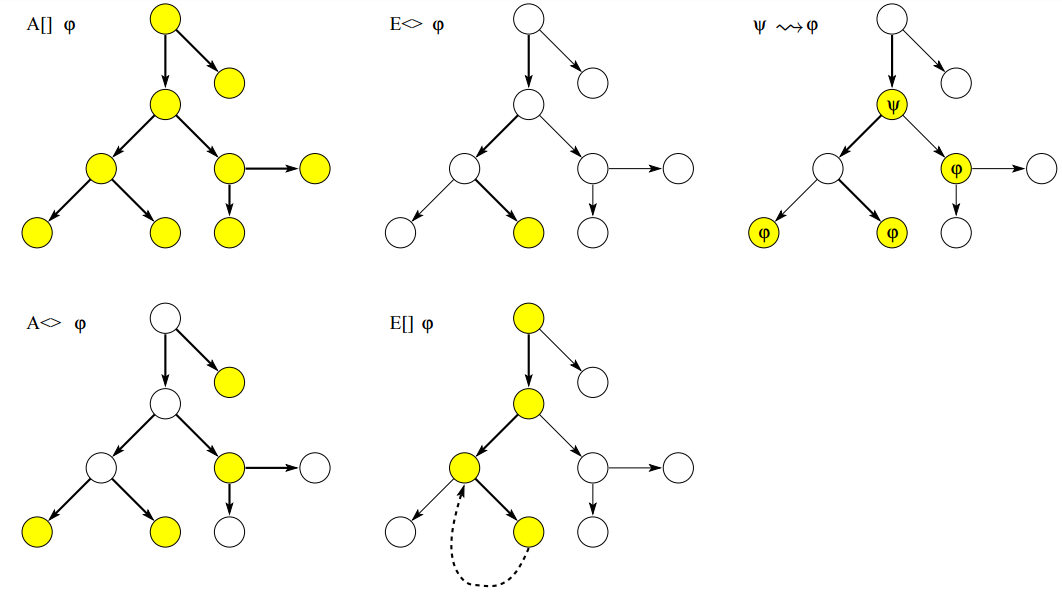
\includegraphics[width=0.9\textwidth]{queries.PNG}
\caption{Illustration of the different property verification queries in UPPAAL. Taken from~\cite[p. 8]{upptut}}.
\label{fig:query}
\end{figure}

\paragraph{Probability estimation}
UPPAAL SMC extends the capabilites of UPPAAL, in a way that allows us to reason about a model in terms of not only "yes" and "no", but also the \textit{probability} a model has of entering a certain state. An example could be determining the probability of a model of a Java bytecode program reaching a state of termination. To allow this, UPPAAL SMC extends regular queries, described earlier, to include probabilities. A query which asks the probability that \textit{some} path in a model of the program in \cref{lst:example} can finish within $100$ time units without an operand stack fault and exceptions occurring, would look as follows\\
\ch{fix description of query from old example}
$$\texttt{Pr\relax[bound\relax] ($\varphi$)}$$
where \texttt{bound} denotes a bound for a simulation run, within which a property, $\varphi$ is to be verified. A bound can be defined in three ways~\cite[p. 402]{smc}

\begin{itemize}
\item implicitly by time by specifying $\leq M$, where $M$ is a positive integer.
\item explicitly by cost with $x \leq M$ where $x$ is a specific clock.
\item by number of discrete steps with $\# <= M$. 
\end{itemize}

UPPAAL SMC will then calculate the probability of this query being true within a certain confidence, e.g. $\relax[0.689, 0.699]$ indicating $68.9$ to $69.9\%$ probability that the query is satisfied within $x$ runs.
\ch{do we need refs for this paragraph?}
